Este módulo abarca los procesos de distribución equilibrada de clases, visualización de secuencias, conteo de palabras y creación de la bolsa de palabras del conjunto de datos final. Además, se encarga del manejo de embeddings y de la creación, entrenamiento y evaluación de los modelos de redes convolucionales. Este módulo contiene las siguientes secciones:

Entrenamiento de Modelos

La carpeta entrenarmodelos almacena los siguientes archivos:

\begin{itemize}

\item creando\_dataset.py: Se encarga de la división de los conjuntos de datos en subconjuntos para el entrenamiento, la validación y la prueba, asegurando que cada una de las tres clases esté representada de la mejor manera para el entrenamiento de los modelos. También permite la visualización del estado del conjunto de datos, como el tamaño de secuencias y la bolsa de palabras. Ver figura \ref{fig:uml7}.

\begin{figure}
	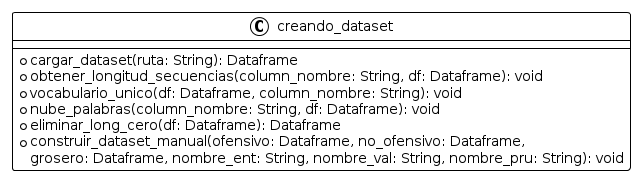
\includegraphics[width=0.65\textwidth]{capitulo5/figuras/fig7.png}
	\caption{Clase creando\_dataset}
	\floatfoot{Fuente: Elaboración propia, generado con PlantUML}
	\label{fig:uml7}
\end{figure}

\item preparar\_datos.py: Recibe el conjunto de datos en formato .CSV mismo que contiene comentarios textuales y sus etiquetas correspondientes. Convierte estos datos a listas para realizar procesos de tokenización, padding, carga de embeddings y procesamiento de embeddings, después de establecer los hiperparametros necesarios como el tamaño máximo de secuencia, el número máximo de palabras y la dimensión de los embeddings, además se crean métodos para el armado de la capa de embedding, compilación, entrenamiento, evaluación y graficación de los modelos Ver figura \ref{fig:uml8}.

\begin{figure}
	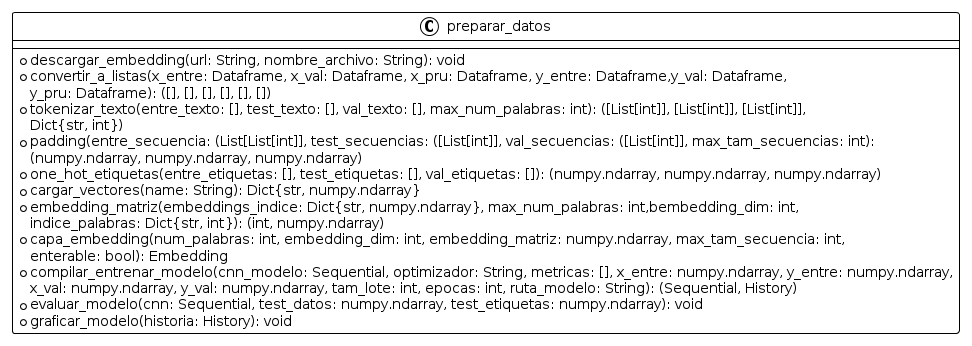
\includegraphics[width=0.65\textwidth]{capitulo5/figuras/fig8.png}
	\caption{Clase preparar\_datos}
	\floatfoot{Fuente: Elaboración propia, generado con PlantUML}
	\label{fig:uml8}
\end{figure}

\item cnn\_tres.py: Crea los modelos de redes convolucionales propuestos con una arquitectura base de tres capas. Ver figura \ref{fig:uml9}.

\begin{figure}
	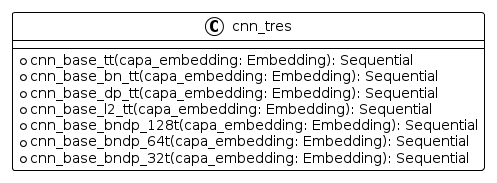
\includegraphics[width=0.65\textwidth]{capitulo5/figuras/fig9.png}
	\caption{Clase cnn\_tres}
	\floatfoot{Fuente: Elaboración propia, generado con PlantUML}
	\label{fig:uml9}
\end{figure}

\item cnn\_four.py: Crea los modelos de redes convolucionales propuestos con una arquitectura base de cuatro capas. Ver figura \ref{fig:uml10}.

\begin{figure}
	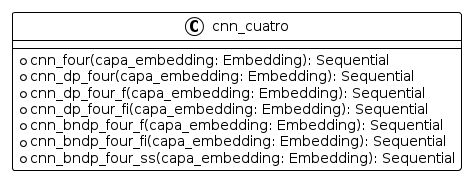
\includegraphics[width=0.65\textwidth]{capitulo5/figuras/fig10.png}
	\caption{Clase cnn\_cuatro}
	\floatfoot{Fuente: Elaboración propia, generado con PlantUML}
	\label{fig:uml10}
\end{figure}

\item cnn\_dos.py: Crea los modelos de redes convolucionales propuestos con una arquitectura base de dos capas. Ver figura \ref{fig:uml11}.

\begin{figure}
	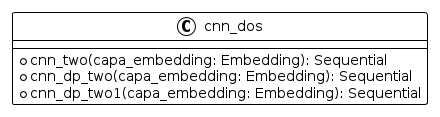
\includegraphics[width=0.65\textwidth]{capitulo5/figuras/fig11.png}
	\caption{Clase cnn\_dos}
	\floatfoot{Fuente: Elaboración propia, generado con PlantUML}
	\label{fig:uml11}
\end{figure}

\end{itemize}

Para la carga de embeddings, se utilizó la versión paga de Colab, debido a la necesidad de usar una mayor capacidad de memoria RAM. Las dimensiones de las estructuras utilizadas para la entrada y salida de las capas de embedding, capas de convolución, capas de max-pooling, etc., se detallarán más adelante.

Para cada modelo propuesto, se guarda una copia en cualquier época durante el entrenamiento en la que la pérdida del conjunto de validación disminuya. Además, para mayor comodidad, se almacena todo el historial de entrenamiento de cada modelo, permitiendo visualizar su avance y realizar comparaciones con otros modelos.
